%\subsection{<Name der Funktion des Teilgraphen, bsp: Eingabeknoten / Pipelinequellen>}
	
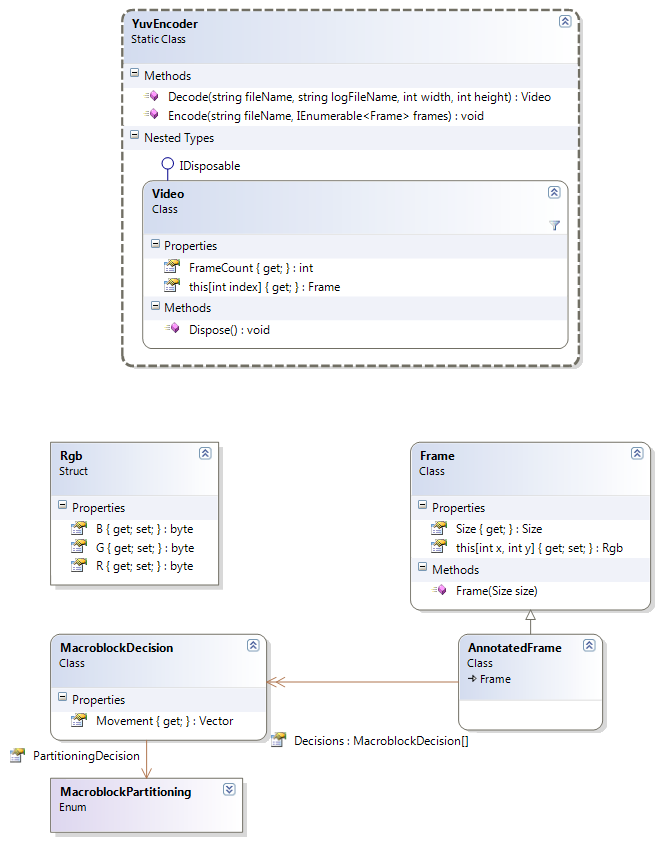
\includegraphics[width=\textwidth]{YuvKA.VideoModel/videomodel.png}
UML-Diagramm, welches die Klassen darstellen, die die unterschiedlichen Framearten bilden, einschließlich ihrer Hilfsklassen. Auch dargestellt ist die Klasse \name{YuvEncoder} mit der inneren Klasse \name{Video} die Videos vom YUV-Format ins RGB-Format umwandelt, mit der das Programm intern arbeitet.

\subsubsection{YuvKA.VideoModel.YuvEncoder}

\begin{verbatim}
public static class YuvEncoder
\end{verbatim}

\paragraph{Beschreibung}~\\
Die Klasse \name{YuvEncoder} bietet die Funktionalität, Videos die im YUV-Format eingegeben werden, ins RGB-Format umzuwandeln, damit das Programm damit arbeiten kann. Desweiteren wandelt es die manipulierten Videos vom RGB-Format ins YUV-Format um, damit sie abgespeichert werden können.

\paragraph{Typmember}
\begin{itemize}

\method{Decode}
	\begin{verbatim}
	public static Video Decode(string fileName, string logFileName, int width, int height)
	\end{verbatim}
	Wandelt das im \name{fileName} angegebene YUV-Video ins RGB-Format um, das interne Format des Programms. 

\method{Encode}
	\begin{verbatim}
	public static void Encode(string fileName, IEnumerable<Frame> frames)
	\end{verbatim}
	Wandelt das als RGB-Frameliste angegeben Video ins YUV-Format um und speichert es unter \name{fileName}. 

\end{itemize}
\setcounter{secnumdepth}{4}
\paragraph{YuvKA.VideoModel.YuvEncoder.Video}
\setcounter{secnumdepth}{3}
\begin{verbatim}
public class Video : IDisposable
\end{verbatim}

\paragraph{Beschreibung}~\\
Die Klasse \name{Video} bietet die Funktionalität, dass sie die vom \name{YuvEncoder} umgewandelten Videos als Videostream hält.

\paragraph{Typmember}
\begin{itemize}

\field{stream}
	\begin{verbatim}
	Stream stream;
	\end{verbatim}
	Hält das eingegebene Video als Array fest.

\property{FrameCount}
	\begin{verbatim}
	public int FrameCount { get; }
	\end{verbatim}
	Ruft die Anzahl der \name{Frames} im \name{stream} ab.

\property{this[int index]}
	\begin{verbatim}
	public Frame this[int index] { get; }
	\end{verbatim}
	Ruft den an der Stelle \name{index} abgespeicherten \name{Frame} im \name{stream} ab.

\method{Dispose}
	\begin{verbatim}
	public void Dispose()
	\end{verbatim}
	Schließt den \name{stream} des \name{Video}-Objekt, sodass der allokierte Speicher frei wird.

\end{itemize}

\subsubsection{YuvKA.VideoModel.Frame}

\begin{verbatim}
public class Frame
\end{verbatim}

\paragraph{Beschreibung}~\\
Die Klasse \name{Frame} stellt ein Einzelbild eines Videostreams im RGB-Format dar.

\paragraph{Typmember}
\begin{itemize}

\property{Size}
	\begin{verbatim}
	public Size Size { get; private set; }
	\end{verbatim}
	Ruft die Auflösung des \name{Frames} ab oder legt sie fest.

\property{this[int x, int y]}
	\begin{verbatim}
	public Rgb this[int x, int y] { get; set; }
	\end{verbatim}
	Ruft den Farbwert des \name{Frames} an der Stelle \name{x,y} in RGB ab oder legt sie fest.

\property{Data}
	\begin{verbatim}
	public Rgb[] Data { get; set; }
	\end{verbatim}
	Ruft die einzelnen Farbwerte des \name{Frames} als Array ab oder legt sie fest.

\end{itemize}

\subsubsection{YuvKA.VideoModel.AnnotatedFrame}

\begin{verbatim}
public class AnnotatedFrame : Frame
\end{verbatim}

\paragraph{Beschreibung}~\\
Die Klasse \name{AnnotedFrame} erweitert die Klasse \name{Frame} um die Funktion, Logfiles des Encoders zu halten.

\paragraph{Typmember}
\begin{itemize}

\property{Decisions}
	\begin{verbatim}
	public MacroblockDecision[] Decisions { get; set; }
	\end{verbatim}
	Ruft die Entscheidungen, die der Encoder bei der Kodierung getroffen hat als Array von \name{MacroblockDecision} ab oder legt sie fest.

\end{itemize}

\subsubsection{YuvKA.VideoModel.MacroblockDecision}

\begin{verbatim}
public class MacroblockDecision
\end{verbatim}

\paragraph{Beschreibung}~\\
Die Klasse \name{MacroblockDecision} stellt die Entscheidung dar, die der Encoder bei der Enkodierung eines Makroblocks getroffen hat.

\paragraph{Typmember}
\begin{itemize}

\property{Movement}
	\begin{verbatim}
	public Vector Movement { get; set; }
	\end{verbatim}
	Ruft die Weg, den ein Makroblock bei der Kodierung gegangen ist ab oder legt sie fest.

\property{Decisions}
	\begin{verbatim}
	public MacroblockPartitioning PartitioningDecision { get; set; }
	\end{verbatim}
	Ruft Informationen darüber ab, wenn und falls ja wie sich ein Makroblock, normalerweise ein Block von 16 x 16 Pixeln, sich aufspaltet oder legt sie fest. Außerdem ruft er die Information ab, es sich um einen Intr- oder Infraframe handelt oder legt sie fest.

\end{itemize}
